\chapter{Architettura interna}

In questo capitolo illustriamo l'architettura interna dell'Engine, cioè del
componente software predisposto alla messa in esecuzione dei programmi Blite.

Ricordiamo che nello scenario delineato avremo un Engine per locazione, o se si
vuole per nodo di rete, e su ognuno di questi componenti sarà possibile
installare o rimuovere definizioni di processi Blite. In pratica un engine
gestir\`a un insieme di definizioni, creando da queste istanze di
processi e utilizzerà l'Environment per interagire con gli altri Engine. 
Dall'environment stesso l'engine verrà notificato riguardo l'accadere di
eventi, quali l'arrivo di messaggi indirizzati alle porte delle sue definizioni.

Dal punto di vista logico relazionale abbiamo già individuato le seguenti
macro entità e relazioni

\begin{figure}[!htp]
\begin{center}
  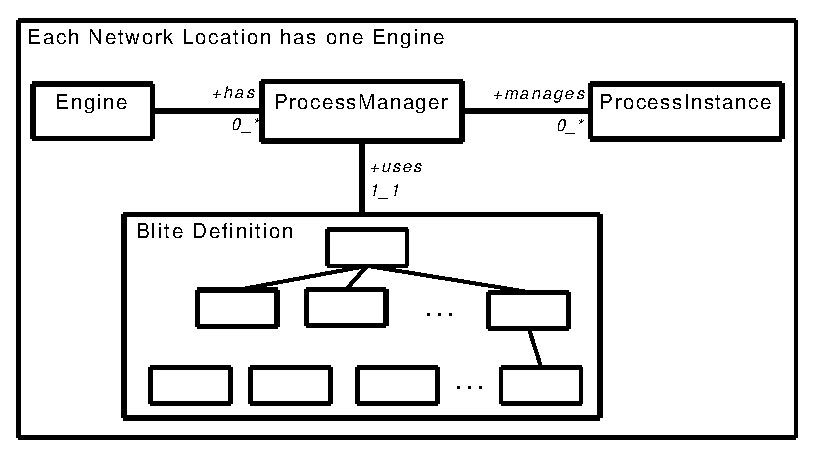
\includegraphics{architettura_interna/dia/engine}
%   \caption[]{
%   	\textsf{{\small Passaggio da reazioni a processi}}
%   }
  \label{fig:1}
\end{center}
\end{figure}

Per ogni definizione istallata sull'engine sarà presente un oggetto istanza
della classe \icode{ProcessManager}, che avrà il compito di gestire, nel loro
ciclo di vita, le istanze di processo derivate dalla definizione.

Prima di entrare nel dettaglio delle scelte architetturali ricapitoliamo quali
sono le caratteristiche peculiari di un sistema che deve gestire programmi per
l'orchestrazione di servizi, in modo che sia pi\`u facile da una parte
comprendere e dall'altra giustificare le scelte fatte.

A nostro vantaggio:
\begin{itemize}
  \item Un Engine contiene in generale un numero contenuto di definizioni, per
  cui non ci interessa la scalabilità rispetto alla quantità di definizioni
  istallate su singolo engine. Tale scalabilità al contrario può essere
  ottenuta aggiungendo altri engine e installando definizioni su engine diversi.
  
  \item  Una definizione (o programma) Blite avendo principalmente funzionalità
  di integrazione avrà una lunghezza generalmente limitata. 
  
  \item Poiché le operazione fondamentali di un programma di questo genere
  sono invocazioni remote, le durate delle esecuzioni hanno ordini di grandezza
  minimi dettati dai tempi caratteristici della rete. Per questo motivo non
  risulta determinante l'efficienza di esecuzione delle operazioni interne di un
  processo. Il nostro engine non necessiterà di una particolare ottimizzazione 
  rispetto all'efficienza di esecuzione interna.
\end{itemize}

al contrario risultano particolarmente critici i seguenti aspetti:
\begin{itemize}
  \item Per ciascuna definizione potrà essere richiesta la creazione di
  innumerevoli istanze. La scalabilità rispetto al numero delle
  richieste remote e quindi di istanze di processo risulta essere un
  prerequisito fondamentale.
  
  \item Se da un lato abbiamo detto che l'efficienza di esecuzione non \`e 
  una aspetto particolarmente critico, dall'altro per\`o ogni attività interna
  necessita di un elevato grado di controllo e tranciabilità. Ogni attività deve
  potere essere eventualmente terminata o abortita. Poiché in generale
  ogni istanza potrebbe avere un immagine persistente o
  perlomeno essere soggetta ad una attività di monitoring, l'engine necessiterà
  di un grado di controllo a livello di singola attività Blite.
\end{itemize}

Tenendo conto di queste iniziali considerazioni sono state fatte alcune scelte
basilari di organizzazione del progetto e l'architettura software \`e stata
basata sulle seguenti specifiche fondamentali:

\begin{enumerate}
  \item La compilazione di una definizione Blite (che eventualmente in un
  ambiente distribuito può essere fatta in fase di deploy) produce un modello
  statico della definizione stessa. Tale modello può essere implementato con una
  struttura ad oggetti che si può pensare di mantenere in memoria presso
  l'engine, tale struttura sarà navigata a runtime per ricavare il
  flusso e la logica di esecuzione. Sempre in fase di deploy l'engine può
  ricavare tutte le informazioni per popolare le strutture dati in cui sono 
  memorizzati i binding fra i nomi delle porte e le definizioni; anche tali
  strutture dati possono essere mantenute in memoria.
  
  \item Le richieste che giungono all'Engine non devono produrre un aumento
  delle risorse complessive mantenute dall'Engine. Ogni istanza di processo nel
  suo svolgersi deve, man mano che procede, rilasciare le risorse di memoria
  acquisite. Anche il numero dei thread complessivo deve essere limitato
  superiormente (generalmente dell'ordine dell'unità). La realizzazione del
  parallelismo di attività deve essere attuata tramite il pattern ``Resources
  Pool''. Ogni Engine deve disporre di un pool di thread con cui eseguire in
  parallelo le attività secondo le definizioni Blite.
  
  \item Il modello di esecuzione deve essere Activity Centric. L'engine deve
  trattare ogni attività secondo una astrazione generica che possa permettere di
  fattorizzare i comportamenti comuni e mantenere semplice e pulita
  l'implementazione della semantica di esecuzione del linguaggio.
\end{enumerate}

%%%%%%%%%%%%%%%%%%%%%%%%%%%%%%%%%%%%%%%%%%%%%%%%%%%%%%%%%%%%%%%%%%%%%%%%%%%%%%%%
%						Modello per l'Attività
%%%%%%%%%%%%%%%%%%%%%%%%%%%%%%%%%%%%%%%%%%%%%%%%%%%%%%%%%%%%%%%%%%%%%%%%%%%%%%%%
\section{Un modello per l'Attività}
A questo punto dopo aver esposto a grandi linee quelle che devono essere le
caratteristiche fondamentali di un engine entriamo nel dettaglio del disegno
della architettura. Nella realizzazione di questa abbiamo scelto di utilizzare
il formalismo degli oggetti e delle classi secondo il consueto paradigma
``Object Oriented''. Inoltre abbiamo preso come fonte di
ispirazione il ``Composite Pattern'' [GANGo4] cercandone una trasposizione nella
problematica dell'esecuzione di un programma Blite. In particolare
l'astrazione di componente \`e stata applicata all'entità attività. Come i
componenti contribuiscono alla realizzazione di un documento o di una
interfaccia utente le singole attività contribuiscono allo svolgersi
dell'esecuzione del processo Blite.
 
Inoltre la tipica struttura gerarchica presente staticamente negli elementi
sintattici di una definizione può essere naturalmente riprodotta a runtime tra
i singoli step di esecuzione, andato a completare l'analogia con le strutture
gerarchiche ad albero tipiche dei tradizionali domini di applicazione del
Composite Pattern. 

L'entità fondamentale del nostro dominio applicativo \`e stata quindi
individuata nella \icode{ActivityComponent} trasposizione a runtime
dell'elemento sintattico Activity definito dalla grammatica di Blite.
Ogni \icode{ActivityComponent} \`e rappresentabile tramite la seguente
interfaccia

\lstinputlisting
[caption={L'interfaccia base del modello di escuzione del Blite Engine},
label=lst:ActivityComponent]
{architettura_interna/java/ActivityComponent.java}

\begin{tabular}{| p{0.3\textwidth } | p{0.6\textwidth}|}
\hline
\icode{ActivityComponent} &  \\
\hline
\small{boolean \textbf{doActivity()}} & \small{\textsf{Costituisce il metodo
centrale per lo svolgersi dell'esecuzione del programma. L'invocazione di tale metodo su
un oggetto attività fa si che essa possa eseguirsi. Il valore booleano
ritornato sarà il discriminate del fatto che il flusso di esecuzione
corrente dovrà o meno interrompersi. Ogni attività oltre che eseguire se
stesa sarà quindi anche responsabile nel guidare il flusso nel passo
successivo. Utilizzando la gerarchia a lei nota imposterà la nuova attività
corrente da eseguire (l'attività padre o un figlio) e ritornerà il valore true. 
Al contraio potrà interrompere il flusso corrente ritornando false.
}}\\
 
& \\
\small{ActivityComponent \linebreak \textbf{getParentComponent()}} &
\small{\textsf{ Tale metodo restituisce se presente l'elemento padre 
dell'attività corrente. In questo modo si realizza la struttura gerarchica fra
i veri componenti dell'esecuzione. }}\\
\end{tabular}
\begin{tabular}{| p{0.3\textwidth } | p{0.6\textwidth}|}
& \\
\small{BltDefBaseNode \linebreak {\textbf{ getBltDefNode()}}} &
\small{\textsf{ Ogni attività componente dell'esecuzione \`e strettamente 
associata ad un elemento sintattico del programma. Con questo metodo ogni 
oggetto attività restituisce il nodo che la definisce nell'albero sintattico
ricavato dal parsing del codice Blite. }}\\

\hline
\end{tabular}
\\

Lo scenario che si va a delineare \`e quindi quello di due strutture gerarchiche
associate: una costituita dall'AST (Abstract Syntax Tree) ricavato dal
parsing del codice Blite, e che come si detto \`e mantenuta nella sua interezza,
l'altra costituita dall'albero dinamico delle ActivityComponent che
realizzano l'esecuzione a runtime. Quest'ultima struttura, una per ogni
istanza, non \`e pero costruita in un unico momento in fase di inizializzazione
del  processo, ma al contrario \`e istanziata man mano che l'esecuzione
procede.  Come già accennato le attività stesse saranno responsabili di creare
i loro successori e di metterli in esecuzione. Inoltre gli oggetti attività
già eseguiti dovranno essere rilasciati il prima possibile in modo da poter 
essere collezionati dal Garbage Collector e rilasciare le risorse di memoria.

\begin{figure}[!htp]
\begin{center}
  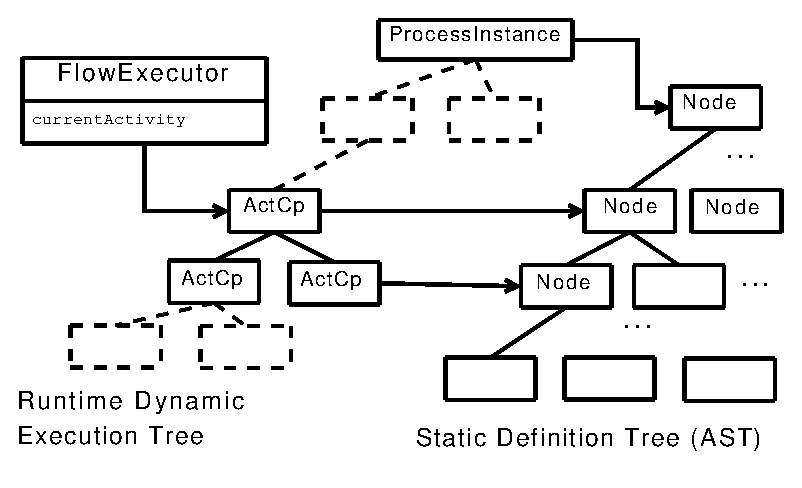
\includegraphics{architettura_interna/dia/tries}
%   \caption[]{
%   	\textsf{{\small Passaggio da reazioni a processi}}
%   }riscrivera
  \label{fig:1}
\end{center}
\end{figure}

Per ogni tipologia di attività prevista dalla grammatica di Blite esisterà
una sotto classe specifica implementante l'interfaccia \icode{ActivityComponent}
e che realizzerà in maniera opportuna, in rispetto della semantica, il metodo
\icode{boolean \textbf{doActivity()}}. Per ottimizzare il disegno e fattorizzare
il codice comune \`e stata ovviamente introdotta una classe astratta
\icode{ActivityComponentBase} da cui ogni altra implementazione di
\icode{ActivityComponent} erediterà le funzionalità comuni di base.

Anche la classe \icode{ProcessInstance}, che modellerà con i suoi oggetti le
varie istanze di processo nell'engine, implementerà l'interfaccia
\icode{ActivityComponent} uniformando la struttura gerarchica di esecuzione.

Le varie istanze di \icode{ActivityComponent} del tipo specializzato verranno
create tramite una classe di Factory \icode{ActivityComponentFactory} che
espone il FactotyMathod \icode{ActivityComponent
\textbf{makeRuntimeActivity}(BltDefBaseNode bltDefNode,\ldots )} 

\lstinputlisting
[caption={ActivityComponentFactory la factory per le ActivityComponent},
label=lst:ActivityComponentFactory]
{architettura_interna/java/ActivityComponentFactory.java}

\begin{center}
\begin{tabular}{| p{0.5\textwidth } | p{0.4\textwidth}|}
\hline
\icode{ActivityComponentFactory} & \\
\hline

\small{
ActivityComponent \linebreak \textbf{makeRuntimeActivity}( 
\linebreak \hspace*{\stretch{3}} BltDefBaseNode bltDefNode, 
\linebreak \hspace*{\stretch{3}} ExecutionContext context, 
\linebreak \hspace*{\stretch{3}} ActivityComponent parentComponent, 
\linebreak \hspace*{\stretch{3}} FlowExecutor executor)} 
& \small{\textsf{ Permette di ottenere istanze opportune di oggetti
\icode{ActivityComponent}. Il parametro bltDefNode individua l'elemento
sintattico che definisce l'attività specifica, in pratica il nodo nel AST.
Il parametro parentComponent l'attività padre nella gerarchia di esecuzione,
mentre gli altri due parametri individuano rispettivamente il contesto di
esecuzione e l'esecutore del flusso in cui l'attività verrà creata. Tali
entità verranno descritte nelle sezioni successive}}\\
\hline
\end{tabular}
\end{center}

In Figura \ref{fig:actclass} viene riportato un diagramma di classe
abbastanza dettagliato per le entità \icode{ActivityComponent}.

\begin{figure}[p]
\begin{center}
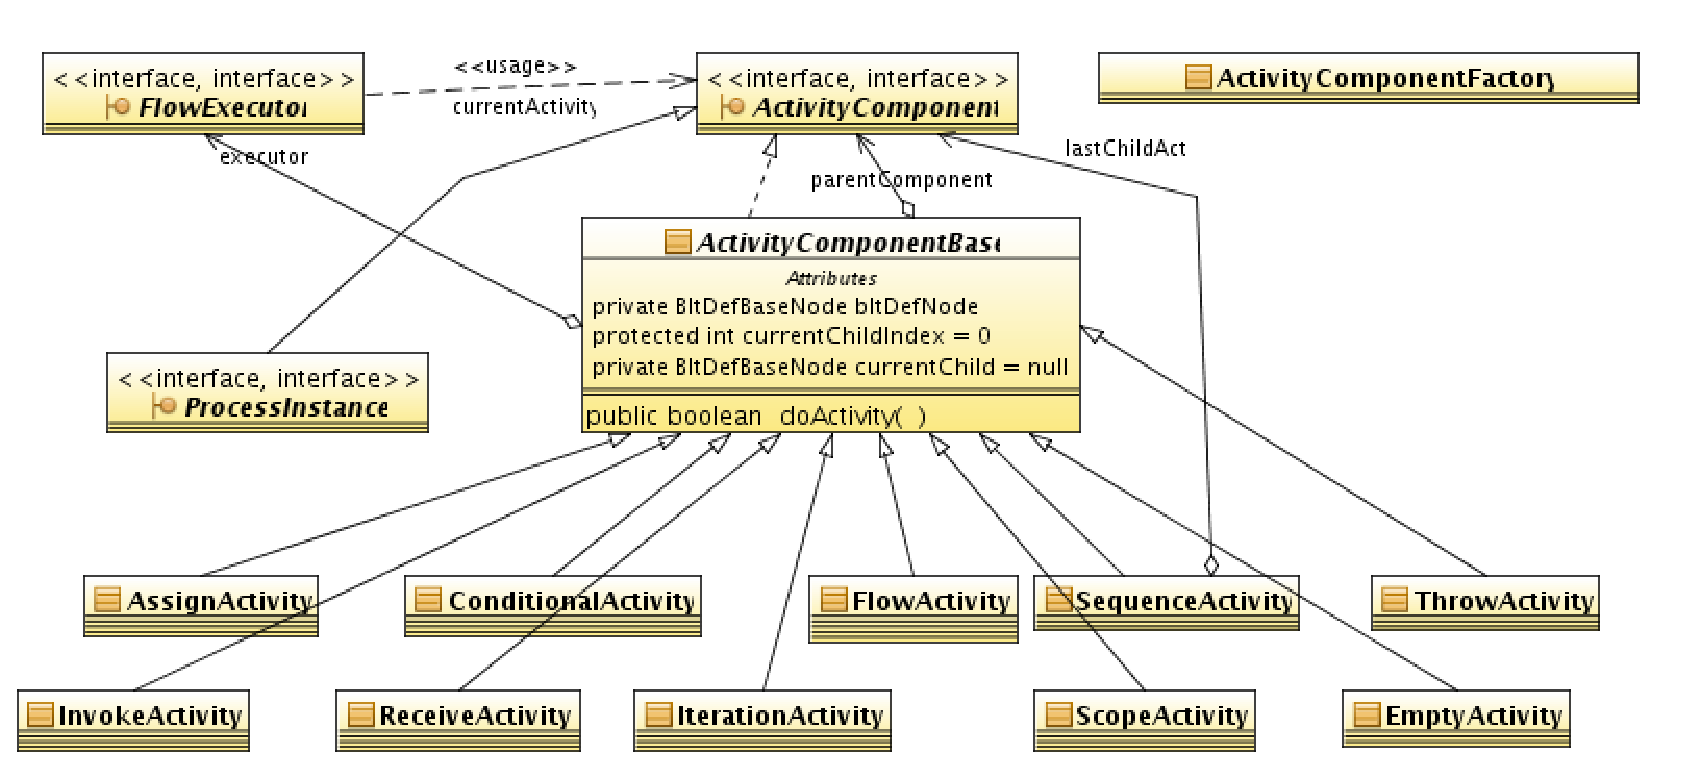
\includegraphics[angle=90,scale=0.80]
{architettura_interna/dia/actclass}
\caption[Gerarchia delle ActivityComponent]{
   	\textsf{{\small Diagramma di classe per la gerarchia delle
   	ActivityComponent}} }
  \label{fig:actclass}
\end{center}
\end{figure}

% %%%%%%%%%%%%%%%%%%%%%%%%%%%%%%%%%%%%%%%%%%%%%%%%%%%%%%%%%%%%%%%%%%%%%%%%%%%%%%%
% Esecuzione e parallelismo
% %%%%%%%%%%%%%%%%%%%%%%%%%%%%%%%%%%%%%%%%%%%%%%%%%%%%%%%%%%%%%%%%%%%%%%%%%%%%%%%
\section{Esecuzione e parallelismo}
Abbiamo visto come i componenti base per l'esecuzione siano oggetti delle varie
sottoclassi implementanti l'interfaccia \icode{ActivityComponent}, e come
l'esecuzione abbia atto tramite l'invocazione del metodo
\icode{\textbf{doActivity()}} su tali oggetti. A questo punto però dobbiamo
domandarci da chi e in che modo tale metodo sia invocato. Nel rispondere a questa
domanda dobbiamo tenere conto che in un engine verranno eseguite
contemporaneamente molteplici istanze di processo e che inoltre il formalismo
stesso del linguaggio da la possibilità di richiedere l'esecuzione contemporanea
di diverse attività (costrutto flaw). Quindi su ciascun Engine dovranno essere
disponibili più thread per poter realizzare il sufficiente livello di
parallelismo.

Ovviamente si capisce bene che istanziare un nuovo oggetto Thread per ogni nuovo
flusso logico presente sull'engine non sia un approccio assolutamente
vantaggioso. Come già accennato infatti tale politica non sarebbe per nulla
scalabile rispetto al numero delle richieste remote gestite dell'engine; inoltre,
poiché ogni istanza di processo tendenzialmente trascorrerà la gran parte del suo
tempo in attesa di comunicazioni remote\footnote{Come già osservato i tempi di
comunicazione remota sono di ordini di grandezza molto maggiori rispetto alle
operazioni interne per cui ogni istanza nel suo ciclo di vita si troverà ad
occupare realmente la CPU per tempi quasi infinitesimi rispetto ai tempi di
attesa di eventi remoti.}, ci troveremmo con un gran numero di thread in stato
di attesa, con un del tutto ingiustificabile spreco di risorse. Più banalmente
gestire direttamente oggetti Thread \`e un pratica alquanto sconsigliabile
\footnote{Questo \`e ancor pi\`u vero dalla versione 5 in poi di Java, in cui
sono stato introdotti i pacchetti \texttt{java.util.concurrent.*} che mettono a
disposizione un framework ad alto livello che ottimizza e astrae l'uso delle API
a più basso livello per la concorrenza.}, in quanto può portare ad errori di
programmazione o ad Memory Leaks nel caso in cui il ciclo di vita di tali oggetti
non sia sempre ben condotto dal programmatore. Per queste motivazioni si \`e
scelto di utilizzare la tecnica del Pooling per gestire un insieme di Thread a
livello di Engine. Con tale tecnica si isola la gestione della tecnologia di
multitasking e si possono applicare politiche anche molto raffinate capaci di
adattare la quantità di risorse utilizzate al carico di lavoro da svolgere. Nella
implementazione attuale dell'Engine si \`e fatto uso dei thread pool forniti
dalla classe \texttt{java.util.concurrent.Executors} presente nella piattaforma
standard Java 5
 
La scelta che quindi \`e stata fatta per realizzare il sufficiente grado di
parallelismo \`e la seguente: ogni flusso logico attivo presente nelle varie istanze di
processo sarà associato all'entità \icode{FlowExecutor} (tale entità \`e già
comparsa in alcuni diagrammi precedentemente illustrati in questo capitolo, per
cui il lettore avrà già intuito la sua funzionalità). Tali oggetti
presenteranno un'interfaccia che permetterà da un lato di impostare l'attività corrente che
dovrà essere eseguita da uno dei thread del pool, dall'altro di eseguire
effettivamente tale attività.

\lstinputlisting
[caption={I FlowExecutors saranno gli oggetti che realizzeranno i flussi di
esecuzione parallela all'interno dell'Engine }, label=lst:FlowExecutor]
{architettura_interna/java/FlowExecutor.java}

A questo punto quando ci sarà bisogno di creare un nuovo flusso di esecuzione per
l'ActivityComponent \texttt{act} si dovrà creare un nuovo FlowExecutor settarci
\texttt{act} come attività corrente e renderlo disponibile ad un thread per
l'esecuzione. Questo ultimo passaggio verrà realizzato tramite l'interfaccia
dell'Engine che disporrà di un metodo per notificare gli executor pronti per
essere eseguiti e metterli a disposizione del pool di threads

\lstinputlisting {architettura_interna/java/queueFlowExecutor.java}

Inoltre ogni flusso giungerà a conclusione (un istanza di processo termina o un
esecuzione parallela definita in una flow Activity si conclude) e tale evento
dovrà essere registrato e produrre eventualmente altri effetti. Per far si che si
realizzi questa necessità si \`e introdotto il concetto di \icode{FlowOwner}.
Ogni attività che nel suo eseguirsi si troverà a creare nuovi flussi di
esecuzione e quindi oggetti \icode{FlowExecutor}  dovrà implementare
l'interfaccia \icode{FlowOwner} e settare se stessa nel FlowExecutor da lei
creato. In questo modo quando il flusso logico terminerà il FlowOwner potrà
essere notificato di tale accadimento tramite l'invocazione del metodo
\icode{flowCompleted()}.

\lstinputlisting
{architettura_interna/java/FlowOwner.java}

A questo punto \`e lecito domandarsi quando si dovrà considerare terminato un
flusso di esecuzione. In generale si applica il seguente ragionamento. Le varie
\icode{ActivityComponent}, che sono legate in una struttura gerarchica che
riflette la definizione statica del programma, termineranno la loro esecuzione
mettendo come attività corrente nel loro FlowExecutor la propria attività padre
(parentComponent). In accordo con questa osservazione risulta quindi corretto
affermare che flusso di esecuzione può essere considerato terminato dal
FlowExecutor quando questo si troverà ad eseguire come attività corrente proprio
il suo FlowOwner. In questo caso su di esso il FlowExecutor non dovrà invocare il
metodo doActivity() ma il metodo flowCompleted() e fatto questo, dovrà terminare
di eseguire il flusso. Il codice seguente spiega meglio di mille parole la logica
alla base di tutto il modello di esecuzione del Blite Engine; in poche righe \`e
sintetizzata il cuore dell'architettura

\lstinputlisting{architettura_interna/java/FlowExecutorImp.java}

In generale possiamo quindi dedurre le seguenti affermazioni che ci possono
aiutare a sintetizzare delle proprietà invarianti

\begin{itemize}
  \item Un FlowExecutor non invocherà mai il metodo doActivity() del suo
  FlowOwner. Viceversa di questo potrà invocare il metodo
  flowCompleted().
  
  \item Su un oggetto ActivityComponent che implementa anche l'interfaccia
  FlowOwner, il metodo doActivity() verrà invocato dal FlowExecutor dell'attività 
  padre.
  
  \item Su di un oggetto ProcessInstance, che \`e il FlowOwner del flusso
  principale dell'istanza e che \`e l'unica attività senza padre, 
  il metodo doActivity() non verrà mai invocato da nessun FlowExecutor.
  
  \item il metodo doActivity() di una ProcessInstance verra' invocato
  dell'Engine stesso in fase di creazione dell'istanza.
  
\end{itemize}

Oltre a creare, eseguire e terminare flussi sarà anche necessario sospenderne
alcuni già in esecuzione, vedi per esempio il caso dell'attività di ricezione
che deve fermare il flusso corrente in attesa di un evento remoto. In questo
caso l'attività utilizzando l'interfaccia dell'Engine e in particolare il
seguente metodo

\lstinputlisting{architettura_interna/java/addFlowWaitingEvent.java}

potrà mettere in attesa il suo FlowExecutor su di un evento identificato dalla
chiave \texttt{eventKey} e che lei stessa aveva provveduto
precedentemente a ricavare. Fatto questo l'attività ritornerà dal proprio metodo
doActivity() con il valore false, in questo modo il FlowExecutor terminerà
l'esecuzione del Flow corrente. Nel momento in cui il messaggio sarà recapitato,
l'Engine potrà individuare il FlowExecutor tramite la chiave \texttt{eventKey} e
rimetterlo in esecuzione, poiché l'attività corrente di quest'ultimo sarà rimasta
l'attività di ricezione essa potrà riprendere il suo lavoro, consumando il
messaggio e permettendo al suo flusso di esecuzione di continuare. Nella sezione
successiva verrà illustrato nel dettaglio come si realizza la comunicazione e la
notifica degli eventi.

In Figura \ref{fig:flowclass} \`e rappresentato un diagramma di classe che
raffigura fra le altre l'entità il FlowExecutor e FlowOwner e le principali
relazioni che le coinvolgono.

\begin{figure}[p]
\begin{center}
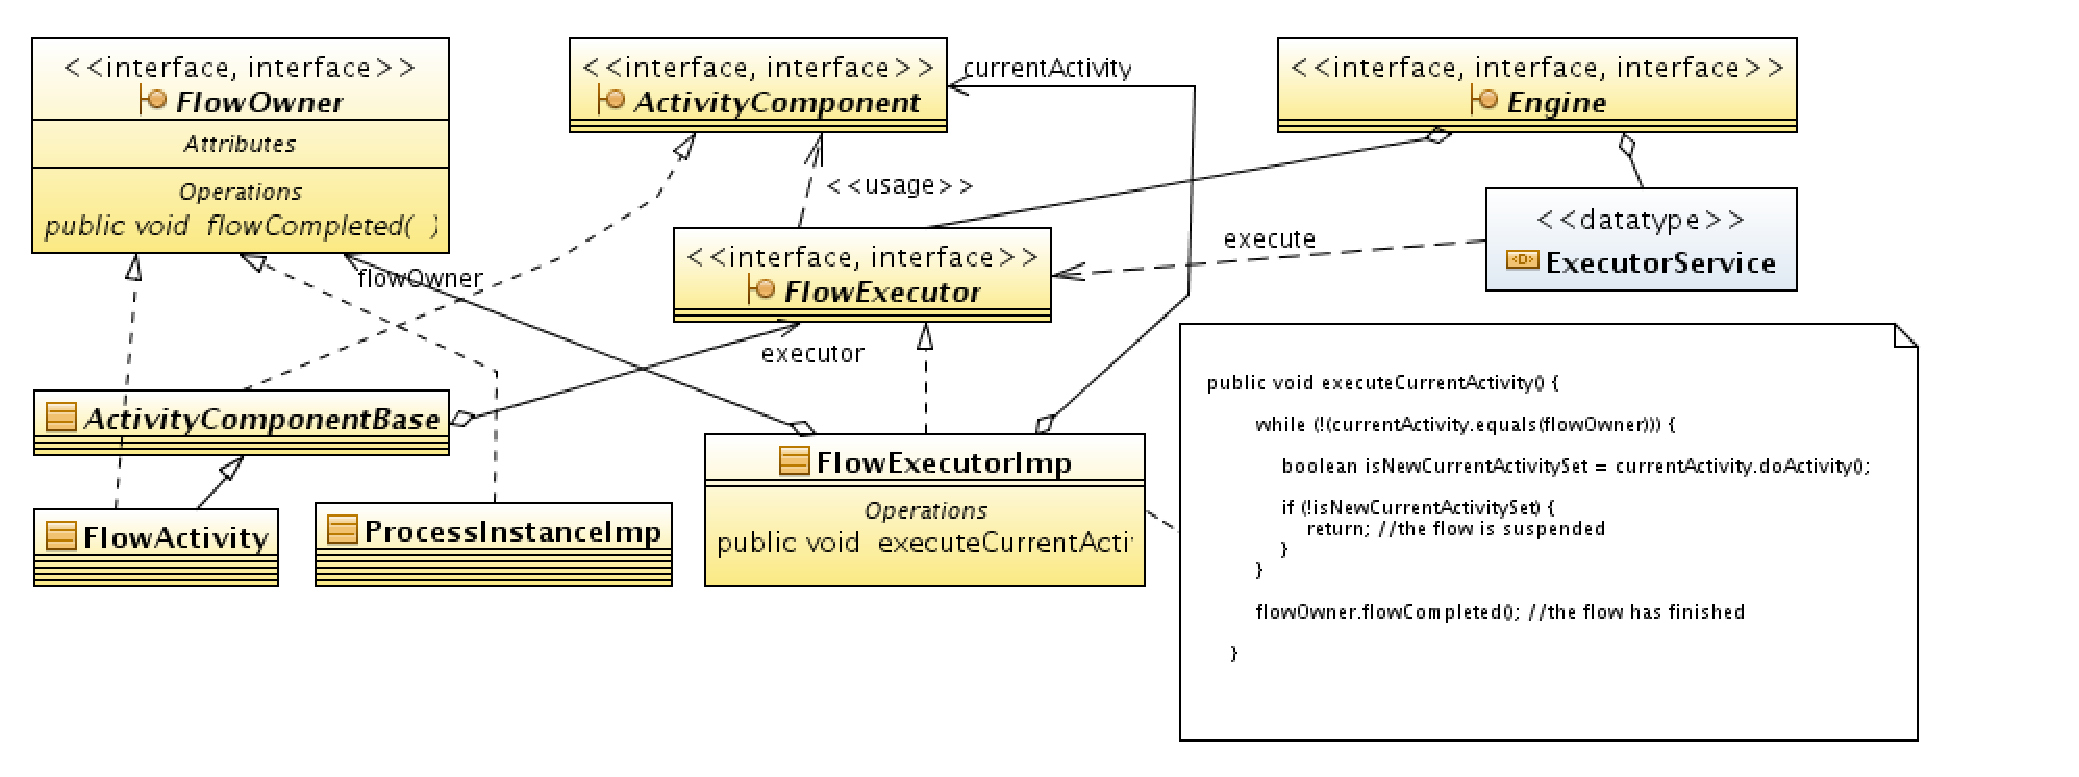
\includegraphics[angle=90,scale=0.75]
{architettura_interna/dia/flowClassDiagram}
\caption[Diagramma di classe FlowExecutor \ldots] {
   	\textsf{{\small Diagramma di classe FlowExecutor, FlowOwner e ThreadPool}} }
  \label{fig:flowclass}
\end{center}
\end{figure}

% %%%%%%%%%%%%%%%%%%%%%%%%%%%%%%%%%%%%%%%%%%%%%%%%%%%%%%%%%%%%%%%%%%%%%%%%%%%%%%%
% EVENTI E COMUNICAZIONE
% %%%%%%%%%%%%%%%%%%%%%%%%%%%%%%%%%%%%%%%%%%%%%%%%%%%%%%%%%%%%%%%%%%%%%%%%%%%%%%%
\section{Comunicazione ed eventi}
Da quanto abbiamo già esposto risulta chiaro che l'esecuzione di un processo \`e
caratterizzata dallo svolgersi di attività interne e l'accadere di eventi
esterni di cui l'attività possono essere in attesa. In generale si può
considerare che gli eventi si generino a livello di Enviroment, e che possano
essere prodotti dall'arrivo di nuovi messaggi verso le porte locali o
dalla notifica degli ack/nok delle invocazioni locali
verso porte remote. Attualmente le funzionalità espresse da Blite non
individuano eventi diversi da queste due tipologie. Nelle engine però si \`e
preferito realizzare un meccanismo generico di notifica di eventi che
soddisfacesse i requisiti attuali del linguaggio ma che non escludesse eventuali
possibilità di estensione verso altre caratteristiche tipiche di BPEL
(comunicazione Request-Response, EventActivity, ecc).

Per l'implementazione dello schema di comunicazione prescelto saranno richieste
le seguenti funzionalità

\begin{enumerate}
  \item A livello di attività o di ProcessManager stesso,
  sarà necessario ricavare una chiave univoca per uno specifico 
  evento\footnote{Si usa qui il termine ricavare e non generare in maniera
  voluta. Le chiavi di evento non sono identificate da oggetti in memoria ma
  hanno una loro entità indipendente
  dagli oggetti che posso essere creati per rappresentarle. Per un esempio le
  chiavi utilizzate per la ricezione saranno costituite dalla coppia
  nomeservizio/nomeoperazione, tele coppia verrà indicata come
  \texttt{portId}.}. I tipi di evento e le regole per generare di volta in
  volta le chiavi verranno esposti di seguito. Per il momento può bastare aver
  chiaro che una chiave individua in maniera univoca una particolare tipologia di evento e all'interno di questa un evento specifico o un insieme
  di eventi gemelli.
  
  \item In un qualsiasi momento al ProcessManager potranno essere notificati
  eventi. In tal caso esso dovrà provvedere a ricavarsi la chiave e a
  memorizzare associativamente l'evento alla chiave per poterlo poi rendere
  disponibile all'attivita' interessate. Il ProcessManager dovrà anche
  provvedere a ``risvegliare'' tutti i flussi di esecuzione che
  eventualmente si sono messi in attesa di quel evento specifico.
   
  \item In un qualsiasi momento e anche più volte nel suo ciclo di vita una
  Attività potrà interrogare l'Engine (o meglio il ProcessManager responsabile
  della sua istanza) chiedendogli se un evento associato ad una particolare
  chiave sia avvenuto. In caso affermativo l'attività potrà consumare l'evento.

  \item Una attività potrà avere la necessità di mettersi in attesa di un
  particolare evento non ancora avvenuto, il tal caso dovrà sospendere il
  suo flusso di esecuzione e notificare questo al ProcessManager
  associativamente alla chiave dell'evento d'interesse. 
\end{enumerate}

% Tali funzionalità serrano rese disponibili nelle diverse interfacce 
% \ldots

In particolare si può vedere come queste funzionalità di base possano essere
utilizzate nel caso dell'attività \icode{ReceiveActivity}, e come
l'attività stessa collabori con il ProcessManager perché si realizzi la
ricezione di messaggi. La \icode{ReceiveActivity} nel suo metodo doActivity
compierà i seguenti passi logici:

\begin{enumerate}
  \item Si ricava la chiave d'evento \texttt{eventKey}. In questo caso
  particolare la chiave sarà di tipo \icode{RequestInComingEventKey} e la sua
  unicità sarà costituita dal \texttt{portId} ( ovvero la coppia 
  serviceName/operationName) della porta su cui si sta eseguendo l'operazione di 
  ricezione. Ovviamente la ReceiveActivity potrà ricavare il \texttt{portId}
  dal nodo della definizione sintattica a lei associata.
  
  \item Si richiede al ProcessManager il set degli eventi associati alla
  \texttt{eventKey}. Se non c'è alcun evento associato si mette in attesa il
  FlowExecutor sull'evento \texttt{eventKey}, si termina ritornando
  \texttt{false}, al contrario si procede con il passo successivo.
  
  \item Si analizza il set degli eventi (che in questo caso possono essere
  identificati con tutti messaggi indirizzati alla porta in questione non
  ancora consumati) per vedere se ce ne possa essere uno indirizzabile alla
  istanza della ReceiveActivity in questione. Questo controllo \`e fatto in
  base alle regole di correlazione (si veda capitolo x). Se un tale messaggio
  non viene identificato si mette in attesa il FlowExecutor sull'evento \texttt{eventKey} e si termina
  ritornando \texttt{false}, al contrario si procede con il passo successivo.
  
  \item Si \`e individuato un messaggio inviato alla porta e alla istanza in
  questione. Si consuma tale messaggio aggiornando lo stato delle variabili
  coinvolte nella ricezione, si imposta la parentComponet come attività
  corrente del FlowExecutor si termina ritornando \texttt{true}.
\end{enumerate}

D'altro canto un oggetto ProcessManager nel metodo \icode{manageRequest( 
ServiceIdentifier service, String operation, MessageContainer
messageContainer)}\footnote{Bisogna notare che
l'invocazione di tale metodo sarà scatenata lato Environment, e che la sua
esecuzione avverrà a carico di un Thread allocato a livello stesso di
Environment e logicamente del tutto indipendente dai thread del pool
dell'Engine.} eseguirà le seguenti operazioni:

\begin{enumerate}
  \item Si verifica che la terna serviceName/operationName/numero parti del
  messaggio identifichi effettivamente una porta valida per la definizione 
  di processo in questione. Se non \`e cosi si notifica una
  situazione di errore all'Environment e questo provvederà ad inviare un NOK al
  processo invocante.
 
 \item Si ricava la \texttt{eventKey} di tipo RequestInComingEventKey associata
 alla porta e con questa si provvede a memorizzare il messaggio in arrivo in una mappa associativa.
 
 \item Se la porta in questione individua una start activity si crea una nuova
 istanza di processo e la si mette in esecuzione, alternativamente 
 
 \item Se la porta non \`e associata ad una start activity si risvegliano tutti
 i FlowExecutor in attesa di eventi individuati dalla \texttt{eventKey}.
\end{enumerate}

Già pensando che le due procedure precedenti saranno eseguite concorrentemente
si capisce che un punto particolarmente critico del meccanismo di
notifica/consumo di eventi sta nel fatto che l'elevato grado di parallelismo
presente possa portare ad una perdita eventi (ovvero non consegna di messaggi).
Quest'ultima \`e di fatto un'ipotesi assolutamente inammissibile e che deve
essere assolutamente evitata. Di fatto essa si manifesterebbe allorché le precedenti
attività parallele fossero sequenzializzate per esempio nel seguente modo

\begin{itemize}
  \item L'\icode{ReceiveActivity} arriva ad eseguire metà del passo 2. Cioè
  ricerca eventi non trovandoli ma non arriva a registrare il FlowExecutor come
  in attesa dell'evento.
  \item Il controllo passa al ProcessManager a cui viene effettivamente
  notificato l'evento di interesse della attività. Esso pero' non trovando
  nessun FlowExecutor in attesa registra l'evento e termina.
  \item Il controllo ripassa all'attività che registra il suo FlowExecutor come
  in attesa. Essendo pero' l'evento già accaduto nessuno a questo punto sarà
  in grado di notificarlo alla nostra ReceiveActivity, di fatto si ha una
  perdita del messaggio.
\end{itemize}

Per evitare questi scenari alquanto deprecabili sono attuabili due strategie.
Una potrebbe essere quella di dotare l'Engine di una procedura temporizzata che
ogni tot di tempo analizzi la mappa degli eventi accaduti e che risvegli
gli eventuali FlowExecutor registrati in attesa di essi. In questo modo il
ProcessManager verrebbe sollevato da quest'ultimo compito e la possibilità di
avere la sequenzializzazione sopra descritta non sarebbe più un problema.
L'altra strategia potrebbe essere quella di eseguire alcuni passi delle
procedure in mutua esclusione, di fatto realizzare due sezioni critiche su un
medesimo semaforo; la prima per la ReceiveActivity dovrebbe comprendere i passi
2 e 3 mentre quella per il ProcessManager raggruppare i passi 2 e 4, o nel caso
della creazione di una nuova istanza i passi 2 e 3.

Per semplicità di realizzazione, e poiché ad una analisi poco più attenta si
capisce che di un certo grado di sincronizzazione non si possa fare a meno\footnote{Se
non altro l'accesso alle strutture dati deve essere sincronizzato fra i vari
thread.}, si \`e scelto di implementare la seconda strategia. Di fatto si \`e
scelto la possibilità di realizzare una sincronizzazione a livello di
definizione di processo. Il ProcessManager esporrà il seguente metodo

\begin{lstlisting}
/**
* Provides a lock at Process definition Level
* 
* @return Object. This object is used to get a lock at process definition level.
*/
public Object getDefinitionProcessLevelLock();
\end{lstlisting}

che restituisce un oggetto che potrà essere utilizzato per sincronizzare un
istanza di processo con il ProcessManager, ma anche le diverse istanze fra di
loro. Tele necessità \`e evidente in quanto ci saranno strutture dati (ad
esempio la mappa che mantiene gli eventi/messaggi per le porte) che saranno
condivise fra le diverse istanze di una definizione di processo. In un certo
modo si può pensare che le diverse istanze siano in ``race'' su tali eventi
nel limite di quelle che sono le regole di correlazione stabilite dal
linguaggio.
\\

Lo schema di comunicazione di Blite risulta semplificato rispetto al modello
proposto da BPEL. In Blite sono possibili solamente invocazioni asincrone, in
cui una istanza invoca una operazione remota con degli input senza attendere
nessuna risposta, il risultato dell'elaborazione sarà reso disponibile
all'invocante tramite una successiva ricezione sfruttando il meccanismo della
correlazione. 

E' stato scelto di realizzare tale schema di comunicazione applicativa tramite lo
schema più semplice di comunicazione infrastrutturale, ovvero lo
schema \emph{One-Way} (o se si preferisce \emph{In-Only} secondo la terminologia
del WSDL 2.0 http://www.w3.org/TR/2004/WD-wsdl20-extensions-20040803/ ). Tale
schema può essere rappresentato nell'ambito della nostra architettura come in
Figura \ref{fig:oneway}. In pratica un'istanza consumer invocherà tramite una
\texttt{request} una porta presso un Engine remoto, provider del servizio
richiesto. Questo dopo aver verificato la disponibilità della porta richiesta e
la conformità formale del messaggio in arrivo rispetto alla stessa, invierà un
\texttt{status-done} (acknowledgment) al richidente, il quale potrà continuare
la sua esecuzione. Al contrario se si sarà verificato un qualche problema un
\texttt{status-error} verrà recapitato al consumer; questo potrà esser fatto
dall'Engine remoto ma anche dall'environment locale stesso qualora si arrivasse
allo scadere di certo timeout senza aver ricevuto alcuno status di risposta (caso
quest'ultimo in cui il provider risulta non raggiungibile). Da notare come tale
schema di comunicazione realizzi un modello di cooperazione dei servizi asincrono
secondo quanto specificato dalla semantica Blite. Il consumo e l'elaborazione del
messaggio da parte di una istanza provider sarà eseguito in maniera del tutto
indipendente, in termini di dipendenze temporali, e quindi anche eventuali errori
nella elaborazioni della richiesta non verranno comunicate al consumer all'interno
di questa comunicazione.

\begin{figure}[th]
\begin{center}
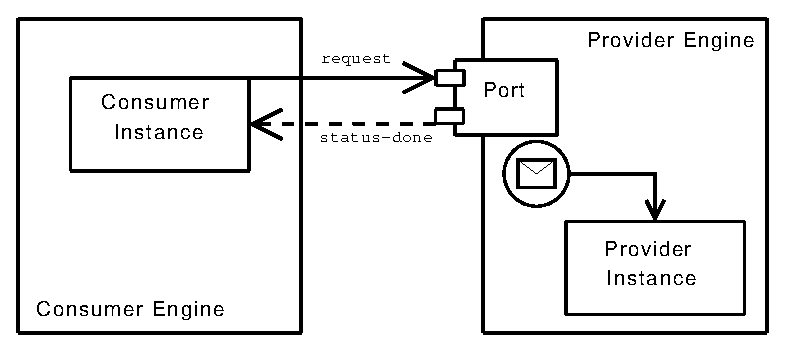
\includegraphics
{architettura_interna/dia/oneway}
\caption[Comunicazione One-Way] {
   	\textsf{{\small Il modello di comunicazione One-Way realizzato dai Blite
   	Engine}} }
  \label{fig:oneway}
\end{center}
\end{figure}


Tele modello ci \`e sembrato il più adatto per poter realizzare i seguenti
comportamenti

\begin{itemize}
  \item Una istanza di processo può invocare operazioni di altri servizi in
  maniera asincrona potendo continuare a svolgere altre attività mentre
  l'elaborazione remota \`e in atto.
  
  \item Se un'istanza invoca un servizio che non esiste, o che \`e
  momentaneamente indisponibile o con modalità non conformi, l'Istanza deve essere notificata
  di tale accadimento.
\end{itemize}

Di fatto questo c'\`e sembrato il giusto compromesso fra una comunicazione
sincrona (che del resto può sempre essere riprodotta) e una comunicazione puramente
``fire-and-forget'' in cui le istanze procedono i maniera totalmente svincolata
senza poter fare nessuna ipotesi sull'esito della comunicazione. Inoltre questo
modello di comunicazione \`e quello che meglio si adatta al binding su
protocolli di trasporto tipo HTTP, in cui ad una richiesta c'e sempre una
risposta del server che chiude la connessione. In HTTP una invocazione remota secondo lo scema
One-Way può essere semplicemente implementata

\begin{itemize}
  \item Il client esegue una \emph{HTTP GET} o \emph{HTTP POST}
  \item Il server risponde con \emph{202 Accepted} nel caso il messaggio possa
  essere accettato.
  \item Il server risponde con un error code della serie 400 o 500 (es. 400 Bad
  Request), nel momento in cui ci sia una qualche problema con la richiesta
  ricevuta.
\end{itemize}


Per concludere questa sezione facciamo vedere come lo schema di comunicazione
One-Way possa essere facilmente realizzato con il modello ad eventi previsto
dalla nostra architettura. Per far questo riportiamo i passi logici eseguiti
dal componente \icode{InvokeActivity}

\begin{enumerate}
  \item Si costruisce il messaggio (\icode{MessageContent}) e si crea un
  identificativo del Service Provider tramite il metodo messo a disposizione
  dell'interfaccia dell'ProcessManager
  \lstset{frame=NONE}
  \begin{lstlisting}
  	/**
     * Resolve PartnerLink at rintime.
     * 
     * @param partnersmDef Static definition of the PartnerLink
     * @param variableScope Runtime variable scope
     * 
     * @return ServiceIdentifier the runtime partner link.
     */
    public ServiceIdentifier resovleParterLink(BLTDEFInvPartners partnersDef, 
											   VariableScope variableScope);
    
  \end{lstlisting}  
  
  \item Tramite il metodo fornito dalla interfaccia del ProcessManager
  \begin{lstlisting}
  	InComingEventKey invoke(ServiceIdentifier serviceId, String operation, 
							MessageContainer messageContainer);
  \end{lstlisting}
  si avvia la comunicazione. Si osservi che il metodo ritorna un oggetto
  \texttt{eventKey} rappresentante una chiave di tipo InComingEventKey. 
  Nel caso particolare sarà un oggetto della classe
  \icode{StatusInComingEventKey}. Questo tipo di chiavi verranno generate a
 livello di Environment negli strati di più basso livello e le
 caratteristiche di unicità dipenderanno fortemente dalla tecnologia di comunicazione
 utilizzata. Per esempio nell'ambito della tecnologia JBI tali chiavi potranno
 coincidere con i \icode{MessgeaExchange}, o in ambito puramente TCP potranno
 essere ricavate dagli identificativi di connessione. In ogni modo a livello di Engine
 \`e possibile astrarre (e lo si deve fare) completamente dalla loro natura e
 utilizzarle semplicemente come identificatori univoci di eventi.
  
  \item In sezione critica sul monitor \icode{DefinitionProcessLevelLock}, si
  prova a consumare l'evento associato all'\texttt{eventKey}, se questo \`e
  effettivamente già disponibile si valuta lo status di ritorno. Se si \`e
  avuto un \texttt{status-done} si termina l'attività mettendo come
  attività corrente del FlowExecutor il parentComponet e si ritorna
  \texttt{true}, se invece si \`e avuto \texttt{status-error} si avvia la
  procedura di errore. Se l'evento associato all'\texttt{eventKey} non fosse
  ancora disponibile si registra il FlowExecutor come in attesa dello stesso e
  si termina il metodo \icode{doAtivity()} ritornando \texttt{false}.
  
  \item Quando l'evento atteso sarà disponibile il FlowExecutor verrà
  risvegliato e l'invokeActivity potrà essere di nuovo messa in esecuzione.
  Questa disponendo già di \texttt{eventKey} potrà rendersi conto di aver
  già eseguito l'invocazione e potrà semplicemente consumare l'evento
  atteso e procedere nell'analisi dello status come descritto sopra. Si deve
  osservare che in questo caso non sarà necessario operare in sezione critica.
\end{enumerate}

% %%%%%%%%%%%%%%%%%%%%%%%%%%%%%%%%%%%%%%%%%%%%%%%%%%%%%%%%%%%%%%%%%%%%%%%%%%%%%%%
% CONTESTI E COMPESAZIONE
% %%%%%%%%%%%%%%%%%%%%%%%%%%%%%%%%%%%%%%%%%%%%%%%%%%%%%%%%%%%%%%%%%%%%%%%%%%%%%%%
\section{Contesti, FaultHandler e Compensazione}

Uno dei costrutti più caratteristici di BPEL \`e senz'altro quello del
contesto, e tale costrutto \`e stato riprodotto con le opportune
semplificazioni anche in Blite e nella versione qui implementata.

Semplificando e rimanendo nell'ambito del linguaggio da noi implementato, un
contesto \`e un raggruppamento logico di attività (di fatto realizzato da
quella che indicheremo con \emph{ContestActivity}), a cui possono essere
associati un \emph{FaultHandler} e un \emph{CompensationHandler}\footnote{Nel
caso in cui il programmatore non codifichi direttamente gli Handler, due
versioni di default sono previste. Il DefaultFaultHandler che prevede
semplicemente la ThrowActivity, in questo modo si realizza la non gestione
dell'eccezione, e il DefaultCompensationHandler con la semplice
EmptyActivity.}. I due handler non sono altro che due attività, la \emph{FaultHandlerActivity} e la \emph{CompensationHandlerActivity} che hanno funzionalità in un certo senso complementari.

\begin{itemize}
  \item La FaultHandlerActivity, \`e un'attività che deve essere eseguita nel
  caso in cui sia sollevato un Fault non gestito 
  durante l'esecuzione della ContestActivity. Di fatto si può pensare che la
  ContestActivity non sia stata completata a causa del verificarsi di una 
  situazione di errore e che a livello del contesto di definizione della 
  ContestActivity stessa si possa gestire l'errore tramite l'esecuzione della 
  FaultHandlerActivity. Di fatto la FaultHandlerActivity entra in gioco nel
  momento in cui la ContestActivity non completa.
  
  \item Al contrario CompensationHandlerActivity entra in gioco solo nel caso
  in cui ContestActivity completi la propria esecuzione con successo, cioè
  senza che si siano verificati errori non gestiti. Di fatto la
  CompensationHandlerActivity può essere vista come la serie di operazioni
  capaci di annullare ciò che \`e stato fatto dalla ContestActivity nel suo
  complesso. 
  Supponiamo di avere un contesto \texttt{c2}, a sua volta
  contenuto in un contesto \texttt{c1} (cioè \texttt{c2} \`e una sotto
  attività di \texttt{a1}, ContestActivity di \texttt{c1}), e che
  \texttt{c2} definisca la ContestActivity \texttt{a2} e la CompensationHandlerActivity
  \texttt{ch1}. Nel caso in cui \texttt{a2} completi con successo la sua
  sua esecuzione, \texttt{ch2} verrà resa nota a \texttt{c1} che la potrà
  utilizzare per annullare gli effetti di \texttt{a2} qualora si verifichi
  qualche successivo errore che impedisca a \texttt{a1} di completare con
  successo.
   
\end{itemize}

Da quanto detto si capisce che l'esecuzione degli handler di un contesto
\texttt{c} \`e strettamente legata al verificarsi di situazioni di errori:
la FaultHandlerActivity \`e lanciata qualora si verifichi un eccezione
nell'esecuzione della ContestActivity di \texttt{c} stesso, la
CompensationHandlerActivity \`e lanciata qualora completato \texttt{c} si
verifichi un errore nell'esecuzione di una qualche attività ``sorella'' di
c\footnote{Nell'ambito della sintassi e semantica di Blite l'espressione
``attività sorella' ha il seguente significato: ``attività che \`e eseguita
nel medesimo contesto del contesto \texttt{c}''.}.

Il sollevarsi di un eccezione oltre a mettere in esecuzione le eventuali
CompensationHandlerActivity e FaultHandlerActivity associate, ha un'altro
effetto: la terminazione di tutti i flussi fratelli o discendenti dei fratelli
del flusso in cui si genera il fault. Per capire gli effetti prodotti dal
sollevarsi di un eccezione si faccia riferimento alla Figura \ref{fig:fault}
dove \`e rappresentato il seguente scenario di runtime

\begin{itemize}
  \item Il contesto base \texttt{C0} definisce il FaultHandler \texttt{fh0}.
  \item L'esecuzione della ContestActivity di \texttt{C0} produce tre flussi di
  esecuzione parallela \texttt{f1}, \texttt{f2} e \texttt{f3}.
  \item Nel flusso \texttt{f1} viene eseguito in contesto \texttt{C1} che
  termina, installando in \texttt{C0} il CompensationHandler \texttt{ch1}.
  \item Nel flusso \texttt{f2} vine creato un nuovo contesto \texttt{C2}.
  All'interno del quale un FlowActivity avvia altri due flussi paralleli
  \texttt{f4} e \texttt{f5}.
  \item Nell'esecuzione del flusso \texttt{f3} viene generato un fault che
  dovrà essere gestito a livello del cotesto \texttt{C0}.
  \item Il fault produce la terminazione de flussi \texttt{f1} e \texttt{f2} e a
  cascata dei flussi \texttt{f4} e \texttt{f5}.
  \item Il fault produce la creazione di un contesto protetto in cui sarà
  eseguito in sequenza la CompensationHandlerActivity \texttt{ch1} e la
  FaultHandlerActivity \texttt{fh0}.
\end{itemize}

\begin{figure}[t]
\begin{center}
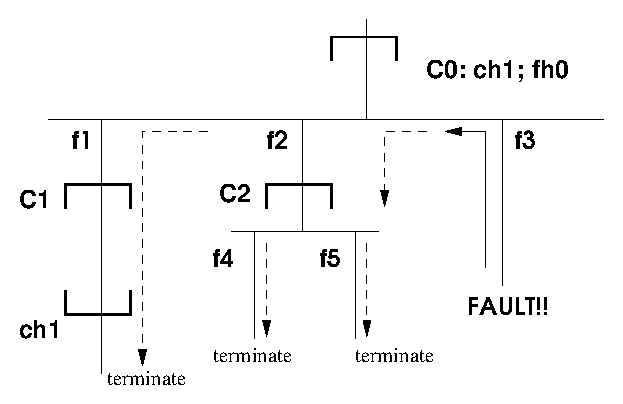
\includegraphics
{architettura_interna/dia/fault}
\caption[Propagazione di una eccezione] {
   	\textsf{{\small Un eccezione sollevata in un flusso di esecuzione produce la
   	terminazione di tutti i flussi paralleli e la conseguente messa in
   	esecuzione di Compensation Handler istallati e FaultHandler definiti nel
   	Contesto padre di flussi.}} }
  \label{fig:fault}
\end{center}
\end{figure}

Come si può vedere dalla Figura \ref{fig:fault} la notifica e gli effetti di
fault si propagano nelle due direzioni opposte nella gerarchia runtime delle
attività. Dalla attività che a scatenato il fault, risalendo i padri, raggiunge
il primo contesto e da questo riscende verso le attività figlie per
interrompere i vari flussi paralleli. Questo andamento di salita e discesa dell'informazione,
legata al sollevarsi di una eccezione, \`e la caratteristica peculiare della
semantica di BPEL e quindi di Blite, e sulla base di questa caratteristica sono
stati disegnati le componenti e le interfacce software dell'engine predisposte alle
gestione dei contesti e delle eccezioni.
\\

L'entità principale prescelta per la realizzazione di meccanismi esposti \`e
stata individuata nel \icode{ExecutionContext}, la cui interfaccia \`e già più
volte comparsa nelle sezioni precedenti. In particolare si \`e visto che un oggetto
conforme a tale tipo era presente nella segnatura del metodo
\icode{makeRuntimeActivity()} della classe
\icode{ActivityComponentFactory}. Difatti ogni oggetto ActivityComponent
nascerà all'interno di un contesto di esecuzione ExecutionContext.
Le classi concrete implementati l'interfaccia ExecutionContext saranno tre, come
si vede dalla Figura \ref{fig:cntxclass}: la \icode{ProcessInstanceImp},
la \icode{ScopeActivity} e la \icode{ProtecedScope}. Ogni istanza di
processo infatti costituirà il contesto base per ogni esecuzione e all'interno
di esso le varie attività ScopeActivity andranno a realizzare dei sottocontesti. Un discorso a
parte invece merita il terzo tipo ProtecedScope, che permetterà di realizzare
contesti speciali, protetti, in cui come visto dovranno essere eseguiti i Fault
e Compensation Handler. Ancora una volta per fattorizzare i comportamenti
comuni si \`e definito una classe astratta \icode{ABaseContext} in cui sarà
codificata gran parte della specifica dell'interfaccia ExecutionContext.

\begin{figure}[tp]
\begin{center}
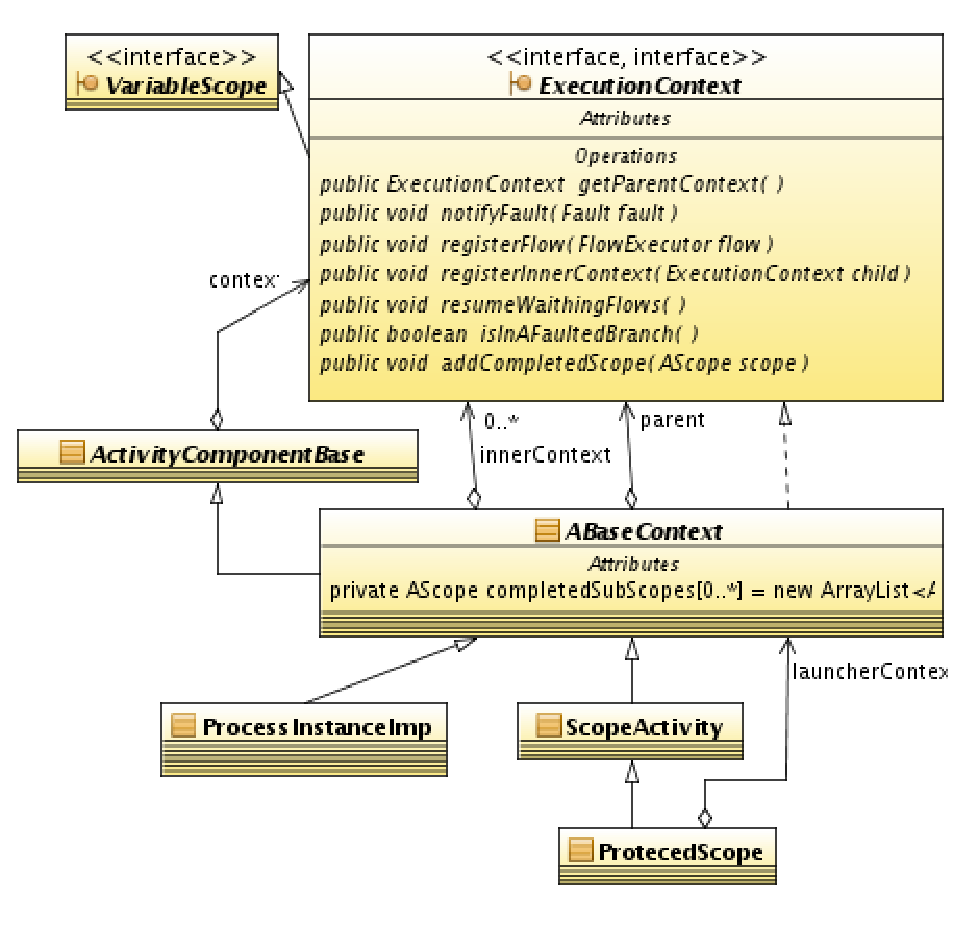
\includegraphics[scale=0.85]
{architettura_interna/dia/cntxclass}
\caption[ExecutionContext Class Diagram]{
   	\textsf{{\small ExecutionContext subclasses}} }
  \label{fig:cntxclass}
\end{center}
\end{figure}

In pratica le varie attività che implementeranno l'Interfaccia ExecutionContext
realizzeranno una sotto gerarchia all'interno della gerarchia principale delle
ActivityComponent. Infatti, a parte la ProcessInstance che costituirà la
ridice dell'albero, oggi ExecutionContext avrà un \texttt{parentContext} ed
eventualmente un insieme di contesti figli.

Analizziamo un po' più nel dettaglio l'interfaccia \icode{ExecutionContext} nei
suoi metodi principali e poi vedremo come questi potranno essere utilizzati per
realizzare la semantica specificata.

\lstinputlisting{architettura_interna/java/ExecutionContext.java}

\begin{tabular}{| p{0.45\textwidth } | p{0.55\textwidth}|}
\hline
\icode{ExecutionContext} &  \\

\hline
\small{ExecutionContext \linebreak \hspace*{\stretch{3}}
\textbf{getParentContext()}} & \small{\textsf{Restituisce il contesto padre
del contesto corrente}}\\

\hline
\small{void \textbf{registerInnerContext}( \hspace*{\stretch{2}} \linebreak  
\hspace*{\stretch{3}} ExecutionContext child)} & \small{\textsf{Aggiunge un
contesto figlio al contesto corrente}}\\

\hline
\small{void 
\textbf{notifyFault}(Fault fault)} & \small{\textsf{Con questo metodo \`e
possibile sollevare eccezioni (faults). Le attività che necessiteranno di
lanciare eccezioni (per esempio la \icode{ThrowActivty}) potranno invocare
tale metodo su il loro ExecutionContext e terminare il loro doActivity
mathod rimettendo in esecuzione il loro parentComponent. L'ExecutionContext
potrà aggiornare il proprio stato per riflettere la situazione di errore.
Con questo metodo ha inizio la propagazione del fault.}}\\

% \end{tabular}
% \begin{tabular}{| p{0.45\textwidth } | p{0.55\textwidth}|}


\hline \small{boolean \textbf{isInAFaultedBranch}()} & \small{\textsf{Questo
metodo sarà utilizzato dalla attività per vedere se nella loro gerarchia di
contesti ne sia presente uno su cui sia stata notificata un eccezione. La
gerarchia in questo caso sarà ispezionata dal contesto padre verso i
predecessori. In tal caso, le attività dovranno collaborare per attuare la
terminazione del proprio flusso, cioè dovranno terminare mettendo in
esecuzione  il proprio parentComponent}}\\


\hline \small{void \textbf{registerFlow}( \hspace*{\stretch{3}} \linebreak
\hspace*{\stretch{3}} FlowExecutor flow)} & \small{\textsf{ Poiché il processo
di terminazione deve coinvolgere tutti i flussi , anche quelli che eventualmente
sono in attesa di eventi, il contesto, una volta notificato del fault, dovrà
risvegliare tutti i flussi creati sotto lui per far si che questi possano
terminare. Ovviamente per poter far questo il contesto dovrà conoscere i flussi
che sono stati creati sotto di lui. Con questo metodo di fatto si realizza
proprio questo, si metterà a conoscenza il contesto sotto cui si sta operando
di ogni nuovo flusso creato. }}\\

% \hline
% \small{void \textbf{resumeWaithingFlows}()} & \small{\textsf{}}\\

\hline
\small{void \textbf{addCompletedScope}(  \hspace*{\stretch{3}} \linebreak
\hspace*{\stretch{3}} AScope scope)} & \small{\textsf{Con questo metodo i
contesti completati con successo potranno registrare nel proprio contesto
padre il loro CompensationHandler per un eventuale esecuzione futura.}}\\

\hline
\end{tabular}
\\

Come abbiamo già osservato si \`e scelto un modello di esecuzione 
Activity Centric, nel senso che le varie attività saranno totalmente
responsabili nel realizzare la loro esecuzione, ma anche nel collaborare per far
sì che i flussi globali dei processi evolvano secondo quanto specificato dalla
semantica. Nell'ambito della terminazione questo concetto si esemplifica nel
fatto che ogni attività (con la sola esclusione \emph{short-live activities})
ogni qualvolta si trovi ad eseguirsi, dovrà per prima cosa verificare di
se si stia trovando nella discendenza di un contesto fallito (questo potrà
essere verificato invocando il metodo \icode{isInAFaultedBranch()} del proprio
ExecutionContext). In caso di risposta positiva l'attività dovrà collaborare
alla terminazione del proprio flusso di esecuzione, cioè dovrà settare il
proprio parentComponent come attività corrente del FlowExecutor e ritornare
immediatamente dal metodo doActivity con il valore true. In questo modo con un
processo a catena il flusso corrente raggiungerà il FlowOwner e potrà così
terminare.
\\

Di fatto la ricerca di un fault a ritroso nella gerarchia di contesti può
semplicemente essere fatta implementando il metodo isInAFaultedBranch() secondo
il seguente algoritmo ricorsivo\footnote{Quella qui presenta \`e
l'implementazione fornita dalla classe ABaseContext ereditata anche per i
contesti ProcessInstaceImp e ScopeActivity. Come si vedrà invece il contesto
ProtecedScope fornirà una riscrittura di questa implementazione, per garantire
la protezione delle esecuzione.}.

\begin{itemize}
  \item Se lo stato corrente del contesto \`e uguale a \texttt{FAULTED} (cioè
  sul contesto \`e stato notificato direttamente un fault) si ritorna
  \texttt{true}. Altrimenti si procede al passo successivo.
  \item Se il contesto non ha un contesto padre si ritorna \texttt{false}.
  Altrimenti si procede al passo successivo
  \item Ricorsivamente si ritorna il valore ritornato dal metodo 
  isInAFaultedBranch() invocato sul contesto padre.
\end{itemize}

Può essere anche interessante osservare quale possa essere la procedura alla
base dell'implementazione del metodo notifyFault(Fault fault)\footnote{Anche
questa implementazione \`e fornita dalla classe ABaseContext ed \`e conforme
alla semantica dei contesti ProcessInstanceImp e ScopeActivity. Per il contesto
ProtecedScope come si vedrà sarà necessario una piccola modifica.}.

\begin{itemize}
  \item Si setta lo stato interno a \texttt{FAULTED}.
  \item Si invoca sul contesto corrente il metodo \icode{resumeWaithingFlows()}.
  Tale metodo ha un comportamento ricorsivo
  \begin{itemize}
  	\item  Su ogni contesto figlio del contesto corrente si invoca ricorsivamente
  	il metodo resumeWaithingFlows() stesso.
  	\item Si risveglia il ogni flusso di esecuzione registrato nel contesto
  	corrente. Tale operazione viene fatta in sezione critica sul consueto
  	semaforo disponibile a livello si definizione di processo:
	\lstset{frame=NONE}  	
	\begin{lstlisting}
	synchronized (manager.getDefinitionProcessLevelLock()) {
                engine.resumeWaitingFlow(flow);
    }
  	\end{lstlisting}	  	 
  \end{itemize}
\end{itemize}

Le due implementazioni saranno valide sia per i contesti di tipo
ProcessInsatnceImp che per i contesti definiti dalle ScopeActivity. In più il
metodo doActivity() di quest'ultima classe realizzerà un algoritmo del tipo seguente

\begin{itemize}
  \item Se isInAFaultedBranch() \`e \texttt{true}
  	\begin{itemize}
    	\item Se lo stato corrente \`e \texttt{FAULTED}, cioè il contesto \`e
    	stato notificato direttamente di un eccezione, si deve avviare gli Handler
    		 \begin{itemize}
             	\item Si crea una SequenceActivity con la sequenza dei
             	CompensationHandler istallati e con il FaultHandler definito
             	\item Si crea un ProtecedScope in cui si imposta come
             	ContestActivity la SequenceActivity appena creata
             	\item Si setta come attività corrente del FlowExecutor il
             	ProtecedScope e si ritorna \texttt{true}.
             \end{itemize}    
    	\item Se lo stato corrente NON \`e \texttt{FAULTED}, cioè un eccezione
    	\`e stata notificata in un qualche contesto padre
    		 \begin{itemize}
             	\item Si setta lo stato a \texttt{TERMINATED}
             	\item Si imposta come attività corrente sul FlowExecutor la
                parentComponent e si ritorna dal metodo con
                \texttt{true}\footnote{Bisogna osservare che questo
                comportamento \`e conforme alla semantica attuale di Blite in
                cui la terminazione di un contesto coincide con la terminazione
                della sua ContestActivity. In realtà se si volesse essere più
                fedeli alla filosofia BPEL e forse più in linea con le
                aspettative di un ipotetico utente del linguaggio, la
                terminazione di un contesto dovrebbe prevedere la messa in
                esecuzione dei CompensationHandler attualmente istallati nel
                contesto stesso. Questo del resto \`e anche il comportamento
                dei default TerminationHandlers di BPEL.}.
             \end{itemize}
    \end{itemize}    
  
  \item Altrimenti se isInAFaultedBranch() e' \texttt{false}
  	\begin{itemize}
  		\item Se lo stato corrente \`e \texttt{STARTED}, cioè uguale allo stato
  		iniziale all'attivita', il contesto deve iniziare ad eseguirsi
  			\begin{itemize} 
                \item Si setta lo stato a \texttt{RUNNING}
                \item Si mette come attività corrente del FlowExecutor la
                ContestActivity e si ritorna con true.
        	\end{itemize}   
  		\item Se lo stato corrente \`e \texttt{RUNNING} allora la ContestActivity
  		ha completato correttamente la sua esecuzione
  			\begin{itemize} 
                \item Si setta lo stato a \texttt{COMPLETED} 
                \item Si registra il CompensationHandler nel contesto padre
                \item Si imposta come attività corrente sul FlowExecutor la
                parentComponent e si ritorna dal metodo con \texttt{true}.
        	\end{itemize}  		 
	\end{itemize}
\end{itemize} 


Concludiamo questa sezione analizzando il contesto \icode{ProtecedScope}. Come
già detto tale contesto verrà utilizzato per la messa in esecuzione dei
CompesationHandlers e dei FaultHandler di un contesto oggetto di un fault.
La semantica di Blite caratterizza tali contesti, differenziandoli da quelli
definiti dalle ScopeActivity, solo per il fatto che questi siano immuni alla
terminazione o si si vuole parlare in termini della semantica Blite, siano immuni
all'applicazione della funzione  {\sf{end($\cdot$)}}

%\ldots work in progress \ldots
\[
\sf{ end( \, \llparenthesis a \rrparenthesis \, ) = \llparenthesis a
\rrparenthesis }
\]
 
Questa caratterizzazione può essere implementata nel nostro modello andando a
riscrivere il metodo isInAFaultedBranch() nella classe ProtecedScope in modo
tale da evitare la chiamata ricorsiva su i contesti padre. Di fatto
l'implementazione in questo caso seguirà il seguente semplice schema

\begin{itemize}
  \item Se lo stato corrente del contesto \`e uguale a \texttt{FAULTED} (cioè
  sul contesto \`e stato notificato direttamente un fault) si ritorna
  \texttt{true}. Altrimenti 
  \item Si ritorna \texttt{false}.
\end{itemize}

In questo modo l'esecuzione che avviene in un ExecutionContext di tipo
ProtectedScope \`e protetta dai fallimenti che possono avvenire in altri flussi
paralleli. 
\\

L'altra caratteristica della semantica Blite \`e che il ProtecedScope
protegge l'attività interna dai fallimenti esterni, ma non fa il
viceversa, cioè i fallimenti che avvengano all'interno del ProtecedScope vanno
ad impattare il contesto il cui ProtecedScope \`e eseguito. Nel momento in cui il
il ProtecedScope viene creato, in fase di gestione dell'eccezione, il contesto
fallito imposta il proprio contesto padre come contesto padre del
ProtecedScope stesso; a questo punto la ``semi trasparenza''
definita dalla semantica di Blite per il ProtecedScope, si realizza nel momento
in cui il metodo notifyFault(Fault fault) viene riscritto secondo la seguente
logica:

\begin{itemize}
  \item Si setta lo stato a \texttt{FAULTED}
  \item Si invoca lo stesso metodo notifyFault(fault) su parentContext
	\lstset{frame=NONE}
	\begin{lstlisting}
		@Override
   		public void notifyFault(Fault fault) {
        	setSate(ContextState.FAULTED);
        	getParentContext().notifyFault(fault);
    	}
  	\end{lstlisting}   
\end{itemize}

Si può facilmente capire che con questa implementazione il ProtecedScope è del
tutto trasparente per le eccezioni che avvengono al suo interno e che si vanno
ad abbattere direttamente sul contesto padre dove eventualmente possono essere
anche gestite.
